% J-CERT+ final narrative revision. Official PVLDB 2027 / Volume 20 template.
% Template files are unmodified; provenance is in template_source/provenance.json.
\documentclass[sigconf,nonacm]{acmart}
%%% do not modify the following VLDB block %%
%%% VLDB block start %%%
\usepackage{pvldb}
%%% VLDB block end %%%
\renewcommand\vldbdoi{XX.XX/XXX.XX}
\renewcommand\vldbpages{XXX-XXX}
\renewcommand\vldbavailabilityurl{https://github.com/X-BoBoowen/J-CERT-Plus}

\usepackage{amsmath,bm}
\usepackage{booktabs,tabularx,multirow}
\usepackage{algorithm,algpseudocode}
\usepackage{tikz}
\usetikzlibrary{arrows.meta,positioning,fit,calc}
\newtheorem{theorem}{Theorem}
\newtheorem{lemma}{Lemma}
\newtheorem{proposition}{Proposition}
\newcommand{\R}{\mathbb R}
\newcommand{\eps}{\varepsilon}
\newcommand{\norm}[1]{\lVert#1\rVert}
\newcommand{\abs}[1]{\lvert#1\rvert}
\newcommand{\up}{\operatorname{up}}
\newcommand{\down}{\operatorname{down}}
\newcommand{\fl}{\operatorname{fl}}
\newcommand{\sym}{\operatorname{sym}}
\newcommand{\diag}{\operatorname{diag}}
\newcolumntype{Y}{>{\raggedright\arraybackslash}X}
\graphicspath{{figures/}}

\begin{document}
\title[J-CERT+: Certified Full-Catalog Intervention Selection in Signed Graphs]{J-CERT+: Certified Full-Catalog\texorpdfstring{\\}{ }Intervention Selection in Signed Graphs}
\author{Bowen Xue}
\affiliation{%
  \institution{Hangzhou Normal University}
  \city{Hangzhou}
  \country{China}}
\email{15869667756@163.com}
\author{Tianyi Chen}
\affiliation{%
  \institution{Hangzhou Normal University}
  \city{Hangzhou}
  \country{China}}
\email{hi@tychen.cc}
\author{Yuze Xia}
\affiliation{%
  \institution{Hangzhou Normal University}
  \city{Hangzhou}
  \country{China}}
\email{2024210401038@stu.hznu.edu.cn}
\renewcommand{\shortauthors}{Xue et al.}

\begin{abstract}
% P:AB1
Selecting an intervention in a signed graph is a ranking query whose scores can change after each accepted edit. A service must evaluate promising edits and justify its choice against every legal alternative, including candidates it never scores. We present J-CERT+, which separates reusable response summaries from current-catalog coverage. Small endpoint summaries support scoring and certified transfer across versions, while coverage bounds direct numerical work toward contenders. Row-frontier and block access paths cover uniformly weighted insertions on initially missing edges and magnitude-preserving flips of initially negative edges. Gain intervals and checked equalities certify positive, tolerance-optimal accepted edits. In an instrumented comparison on Bitcoin Alpha and OTC, row-frontier access reduces aggregate setup-plus-service time by a factor of 3.79 relative to explicit indexing across 15 matched repetitions on the five completed streams of a six-stream confirmation batch. A separate common-lightweight comparison on the same inputs gives block access 12.56\% lower aggregate cost than row access, exchanging cheaper coverage preparation for greater response demand. Independent full-catalog replay verifies all 30 decisions in two preselected row-frontier requests.
\end{abstract}

\maketitle
%%% do not modify the following VLDB block %%
%%% VLDB block start %%%
\vldbtopmatter
%%% VLDB block end %%%

\section{Introduction}
\label{sec:introduction}

% P:I1
Graph intervention asks which change to a network best improves a global objective, as in link optimization for opinion dynamics or information access~\cite{zhu2021polarization,liu2026accessfairness}. When edits are applied in sequence, each choice changes the problem faced by the next. We study this task under the signed Friedkin--Johnsen model, where fixed input opinions and positive or negative interactions determine the expressed equilibrium~\cite{friedkin1990opinions,zhou2024signedfj}. The objective is equilibrium energy: the squared magnitude of expressed opinions plus weighted signed disagreement. An edit's \emph{gain} is its reduction in this energy. A request asks the service to choose improving edits from a legal catalog, with a specified tolerance and tie order. Certifying such a choice requires evidence about both its gain and its competitors.

% P:I2
The difficulty is that a local edit can change the equilibrium throughout the network. A candidate rejected earlier may become attractive even though its own edge is untouched. On a three-vertex path with two negative edges and only their negative-to-positive flips permitted, the right flip initially increases energy. After the left flip, the right flip decreases energy and becomes the best remaining choice (Proposition~\ref{prop:revival}). The second decision needs evidence valid for the updated state.

% P:I3
This creates a data management problem at the intersection of selective ranked access~\cite{bruno2002webtopk,guo2008querydependent} and incremental analytics~\cite{Koch_2014,Nikolic2014Linview}. Evaluating one contender may require a global linear solve, even though only a few endpoint quantities enter its gain. Meanwhile, allowing every missing edge to be inserted gives a sparse graph a quadratic candidate space. An explicit index materializes that space; streaming avoids the table but repeatedly scans it. Response reuse targets the numerical cost, while bounds on unexamined candidates target the access cost.

% P:I4
J-CERT+ separates the numerical information used to score an edit from the coverage bounds used to choose it (Figure~\ref{fig:system}). The response layer selectively maintains small endpoint summaries and transfers them across edits with certified error bounds. The coverage layer accounts for every legal alternative using bounds valid for the current graph and request. These bounds direct response acquisition toward contenders; the resulting gain intervals in turn sharpen the decision threshold. The service can therefore reuse numerical work while establishing a complete basis for each new choice.

% P:I5
We instantiate this design for positive insertions at a common weight on all initially missing edges and magnitude-preserving flips of initially negative edges. H covers this mixed catalog through ordered insertion rows and an ordered flip list. G first tests whether a flip can exclude all insertions, then uses disjoint insertion blocks when needed. Each path provides complete coverage through its own access structure. Both share the response layer with explicit indexing (D) and bounded streaming (S).

% P:I6
Finite precision connects the access and response layers. J-CERT+ propagates errors in maintained summaries and encloses computed gains in conservative intervals. It compares a proposed winner's lower bound with upper bounds on all rivals, using checked structural equalities to resolve supported ties. Every accepted edit satisfies the same positivity, coverage, and tie requirements, whichever access path supplies the candidates.

% P:I7
Experiments on Bitcoin Alpha and OTC show how the two layers affect complete service cost. In the instrumented D/S/H comparison, H reduces aggregate setup-plus-service time by a factor of 3.79 relative to D across 15 matched repetitions on five completed confirmation streams. A separate common-lightweight comparison on the same inputs gives G 12.56\% lower aggregate cost than H: cheaper coverage preparation offsets greater response demand. Independent full-catalog replay verifies all 30 decisions in two preselected H requests.

\begin{figure*}[t]
\centering
% Preserve the supplied PNG. The two inter-layer labels are corrected in the
% typesetting layer: contenders flow down; certified gain bounds flow up.
\begin{tikzpicture}
\node[anchor=south west,inner sep=0] (figone) at (0,0)
  {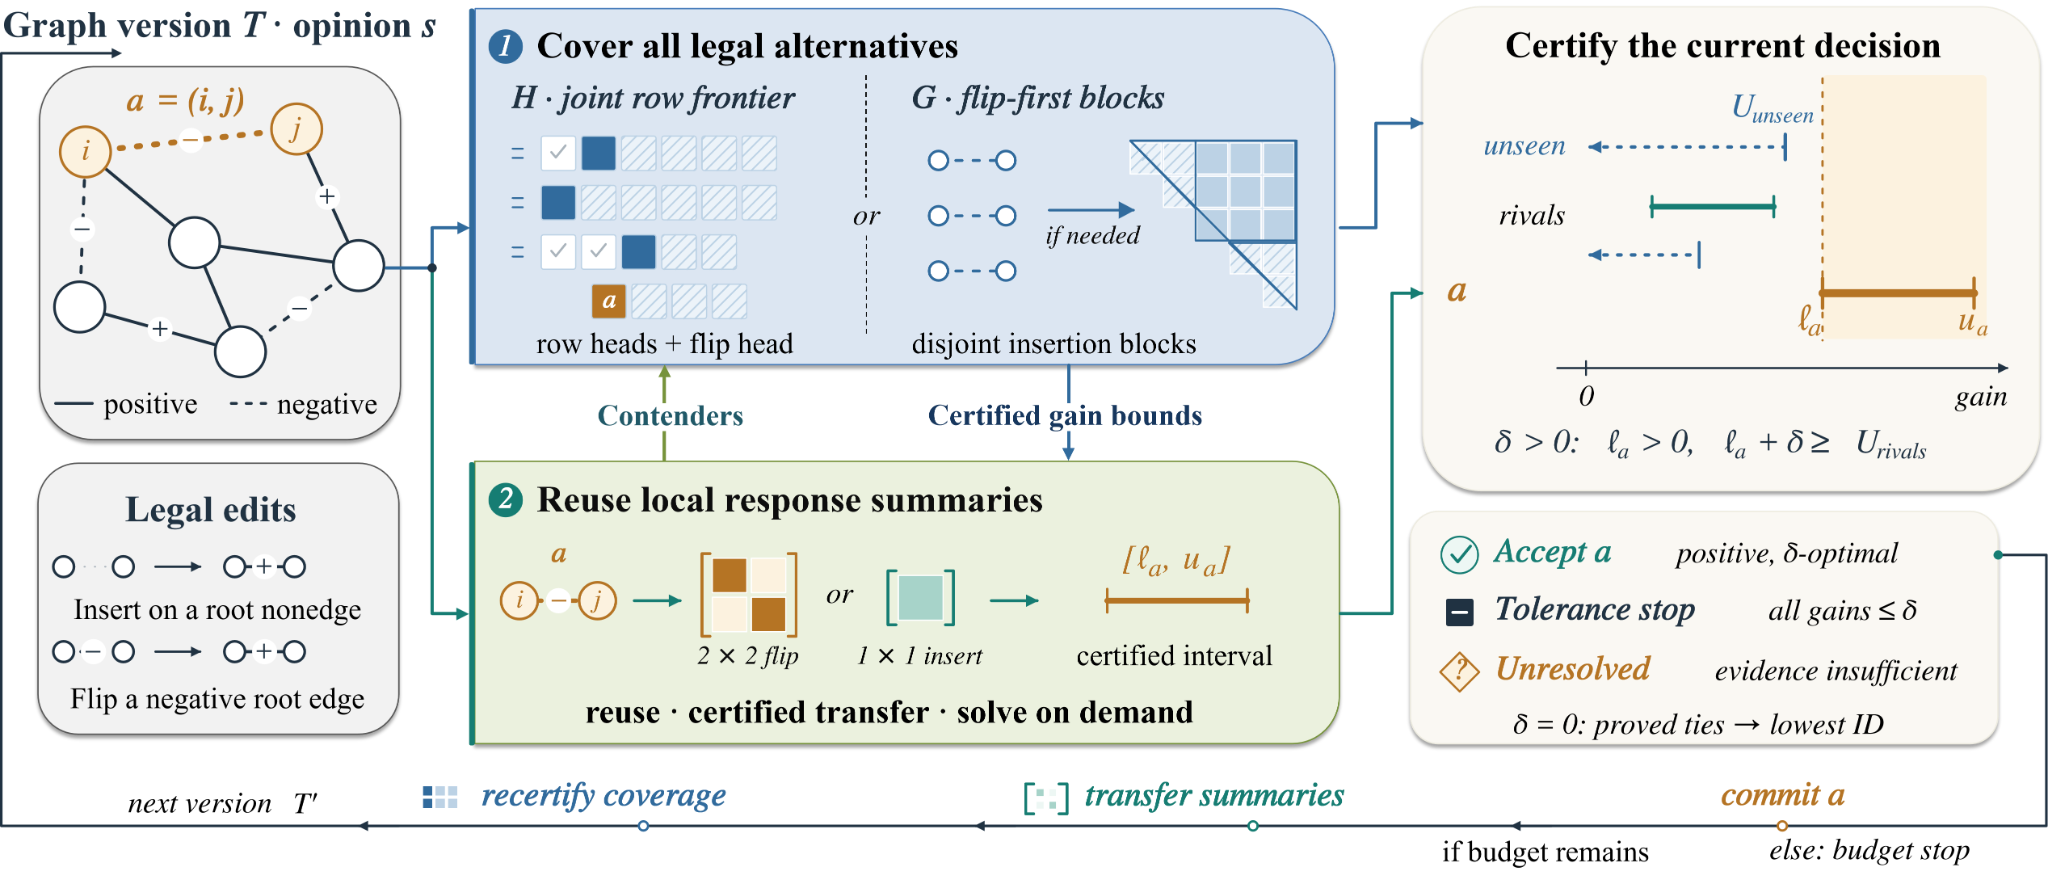
\includegraphics[width=\textwidth]{user_originals/fig1.png}};
\begin{scope}[x={(figone.south east)},y={(figone.north west)}]
\fill[white] (0.2441,0.4994) rectangle (0.6006,0.5420);
\node[font=\bfseries\fontsize{7.2}{8}\selectfont,text=teal!65!black,inner sep=0]
  at (0.3242,0.5207) {Certified gain bounds};
\node[font=\bfseries\fontsize{7.2}{8}\selectfont,text=blue!45!black,inner sep=0]
  at (0.5215,0.5207) {Contenders};
\end{scope}
\end{tikzpicture}
\caption{Current coverage and reusable responses cooperate to certify each edit. H's row frontier or G's block cover identifies contenders; local responses return certified gain bounds. At graph version $T$ with opinion $s$, $[\ell_a,u_a]$ encloses candidate $a$'s gain, $U_{\mathrm{rivals}}$ bounds every other legal candidate, including unseen ones, and $\delta$ is the selection tolerance. An accepted edit advances the version, transfers summaries, and re-establishes coverage while budget remains.}
\Description{A signed graph and its legal edits feed two cooperating layers. Coverage sends contenders to the response layer, which returns certified gain bounds. The current decision combines bounds on unseen candidates and evaluated rivals with a candidate's gain interval. An accepted edit transfers summaries and establishes coverage for the next graph version.}
\label{fig:system}
\end{figure*}


\section{Model and Decision Contract}
\label{sec:contract}

% P:C1
The input opinion and the expressed equilibrium play different roles. Let $G=(V,E,w,\sigma)$ be an undirected simple graph on $n=|V|$ vertices, with positive edge weights $w_e$ and signs $\sigma_e\in\{-1,1\}$. The fixed input vector is $s\in[-1,1]^n$; the equilibrium solves $Az=s$, where the graph determines the operator $A\in\R^{n\times n}$. At the initial, or \emph{root}, graph, interaction strength $\alpha>0$ gives
\begin{equation}
 A_0=I+\alpha\sum_{\{i,j\}\in E}w_{ij}
 (\mathbf e_i-\sigma_{ij}\mathbf e_j)
 (\mathbf e_i-\sigma_{ij}\mathbf e_j)^\top.
 \label{eq:operator}
\end{equation}
Here $I$ is the $n\times n$ identity and $\mathbf e_i\in\R^n$ is the $i$th coordinate vector. The sum is a weighted signed Laplacian~\cite{Kunegis_2010}: a positive edge penalizes the difference between its endpoint opinions, while a negative edge penalizes their sum.

% P:C1a
A finite root catalog $\mathcal C$ assigns at most one action to each unordered pair: insert a positive edge on a root nonedge, or flip a negative root edge to positive while preserving its weight. For candidate $e=\{i,j\}$, write $b_e=\mathbf e_i-\mathbf e_j$, $c_e=\mathbf e_i+\mathbf e_j$, and $\omega_e=\alpha w_e$, using the prescribed insertion weight when $e$ is a nonedge. The operator change is
\begin{equation}
 \Delta_e=\begin{cases}
 \omega_e b_eb_e^\top,&\text{insertion},\\
 \omega_e(b_eb_e^\top-c_ec_e^\top),&\text{flip}.
 \end{cases}
 \label{eq:updates}
\end{equation}
An insertion adds one endpoint direction. A flip replaces one direction by another and is an indefinite rank-two change, with eigenvalues $\pm2\omega_e$ on the endpoint subspace. Scoring a flip must account for both terms.

% P:C2
Let $T\subseteq\mathcal C$ be the committed edits, each used at most once. All candidates at this version are compared using the same input $s$ and current equilibrium $z_T\in\R^n$:
\begin{equation}
 \begin{aligned}
 A_T&=A_0+\sum_{e\in T}\Delta_e,&z_T&=A_T^{-1}s,\\
 \Phi(T)&=s^\top A_T^{-1}s,&g(e\mid T)&=\Phi(T)-\Phi(T\cup\{e\}).
 \end{aligned}
 \label{eq:objective}
\end{equation}
The energy $\Phi(T)$ equals $\|z_T\|_2^2$ plus weighted signed disagreement in the edited graph. It defines the computational objective; the gain compares one edit with its current parent.

% P:C2a
Legality supplies a stability property used throughout the paper. Every fractional operator $A(x)=A_0+\sum_e x_e\Delta_e$, $0\le x_e\le1$, satisfies $A(x)\succeq I$: $A(x)-I$ is positive semidefinite. A partial flip replaces a negative-edge term by a convex combination of negative and positive terms. The full operator $A(x)$ also has diagonal-dominance margin at least one. At a maximum-magnitude coordinate of $v\in\R^n$, this gives $\|A(x)v\|_\infty\ge\|v\|_\infty$. Consequently its induced Euclidean and maximum norms satisfy $\|A(x)^{-1}\|_2\le1$ and $\|A(x)^{-1}\|_\infty\le1$, ensuring a unique equilibrium and bounding numerical solution errors.

% P:C3
With remaining commit budget and additive tolerance $\delta\ge0$, the service may accept $a$ only if
\begin{equation}
 g(a\mid T)>0,\qquad
 g(a\mid T)+\delta\ge\max_{e\in\mathcal C\setminus T}g(e\mid T).
 \label{eq:decision}
\end{equation}
A \emph{tolerance stop} proves that all remaining gains are at most $\delta$; a \emph{budget stop} records exhaustion of the requested commit count. At $\delta=0$, exact maximizers are ordered by a fixed canonical identifier, and the smallest identifier wins. For the implicit catalog, $\mathrm{id}(i,j)=in+j$ for $0\le i<j<n$, with checked signed-64-bit range. Identifiers are computed from endpoints without storing the full list.

% P:C4
To prove a choice, the service combines lower evidence for the proposed winner with upper evidence for its competitors. Write $g_e=g(e\mid T)$. A scored candidate has a certified interval $g_e\in[\ell_e,u_e]$; an endpoint-only exclusion has a valid upper bound $u_e$ and $\ell_e=-\infty$. The remaining, unseen candidates share an upper bound $U_{\rm unseen}$. Empty maxima are $-\infty$. For $\delta>0$, $\ell_a>0$ and
\begin{equation}
 \ell_a+\delta\ge\max\{U_{\rm unseen},\max_{e\ne a}u_e\}
 \label{eq:accept}
\end{equation}
suffice. At $\delta=0$, an earlier identifier requires strict exclusion; a later one permits non-strict domination or certified equality. The aggregate cut $U_{\rm unseen}<\ell_a$ safely excludes unseen rivals of either order. When no positive incumbent exists, a nonpositive upper bound excludes an edit from a positive choice. An unsupported overlap that blocks the decision requires refinement or an \emph{unresolved} result; it cannot be treated as a tie.

\begin{proposition}[A rejected edit can revive]\label{prop:revival}
Consider a three-vertex path with two negative unit-weight edges, $\alpha=1$, intrinsic opinions $s=(1,-3/10,-1/2)^\top$, and a catalog containing only its two flips. The left and right root gains are $1/20$ and $-2/5$. After the left flip, the right gain is $1/10$.
\end{proposition}
\begin{proof}
The root inverse is $\frac18\left(\begin{smallmatrix}5&-2&1\\-2&4&-2\\1&-2&5\end{smallmatrix}\right)$. A left or right flip conjugates it by $\diag(-1,1,1)$ or $\diag(1,1,-1)$, respectively, where $\diag$ forms a diagonal matrix. Evaluating the four quadratic forms gives energies $621/800$, $581/800$, $941/800$, and $501/800$ for neither, left, right, and both flips. Their differences give the stated gains.
\end{proof}

% P:C5
The example shows why exclusions belong to a graph version. The service certifies each current choice in~\eqref{eq:decision}; its optimization scope is the next edit in the sequence. We first identify the response information needed to score a contender, then show how to cover the candidates left unscored.

\section{Selective Response Views}
\label{sec:responses}

% P:R1
An edit changes only one or two endpoint directions, even though its effect on the equilibrium is global. This \emph{low-rank} structure lets us score it through a small system. Write $\Delta_e=U_eJ_eU_e^\top$, with $U_e\in\R^{n\times r_e}$ and rank $r_e\in\{1,2\}$. An insertion uses $U_e=\sqrt{\omega_e}b_e$, $J_e=[1]$; a flip uses $U_e=\sqrt{\omega_e}[b_e,c_e]$, $J_e=\diag(1,-1)$. At a fixed version, abbreviate $A=A_T$ and $z=A^{-1}s$. The quantities needed for scoring are
\begin{equation}
 Y_e=A^{-1}U_e,\quad G_e=U_e^\top Y_e,\quad
 h_e=U_e^\top z,\quad B_e=J_e+G_e.
 \label{eq:gram}
\end{equation}
The full response $Y_e\in\R^{n\times r_e}$ solves $AY_e=U_e$. Its projection onto the edit directions is the \emph{Gram matrix} $G_e\in\R^{r_e\times r_e}$. The vector $h_e\in\R^{r_e}$ projects the equilibrium onto those directions. The \emph{pivot} $B_e$ is the small scoring system, distinct from the full child $A+\Delta_e$. The Gram depends on the graph and edit basis, not on $s$.

\begin{lemma}[Response and Gram transfer]\label{lem:woodbury}
For a legal update $A'=A+UJU^\top$, let $Y=A^{-1}U$, $h=U^\top z$, and $B=J+U^\top A^{-1}U$. The pivot is nonsingular and
\begin{equation}
 \begin{aligned}
 A'^{-1}&=A^{-1}-YB^{-1}Y^\top,\\
 z'&=z-YB^{-1}h,\qquad g=h^\top B^{-1}h.
 \end{aligned}
 \label{eq:woodbury}
\end{equation}
After committing $a$, an unchanged candidate basis has
\begin{equation}
 G'_e=G_e-C_{ea}B_a^{-1}C_{ea}^\top,
 \qquad C_{ea}=U_e^\top Y_a.
 \label{eq:transport}
\end{equation}
\end{lemma}
\begin{proof}
Both the parent $A$ and legal child $A'$ are positive definite. Since $J^{-1}=J$, the determinant identity $\det A'=\det A\det J\det B$ makes $B$ invertible. The signed Woodbury formula~\cite{Hager1989} therefore applies and gives~\eqref{eq:woodbury}. Multiplying that identity on the left by $U_e^\top$ and on the right by $U_e$ yields~\eqref{eq:transport}.
\end{proof}

% P:R2
One winner response can update many stored views. The cross-response matrix $C_{ea}\in\R^{r_e\times r_a}$ uses only $Y_a$'s rows at candidate $e$'s endpoints. After acquiring the winner response or reusing a correctly bound resident block, transferring $m_t$ retained Grams at version $t$ takes $O(m_t)$ local work. A candidate being materialized for the first time requires its own response. Reverse transfer uses the child response and sign matrix $-J_a$.

% P:R3
The implementation removes square roots from response right-hand sides by using exact integer endpoint columns $V_e$, with $U_e=\sqrt{\omega_e}V_e$. Its normalized quantities are $\bar Y_e=A^{-1}V_e$, $\bar G_e=V_e^\top\bar Y_e$, $\bar h_e=V_e^\top z$, and $\bar B_e=J_e/\omega_e+\bar G_e$. They give the same physical gain $g_e=\bar h_e^\top\bar B_e^{-1}\bar h_e$. With $\bar C_{ea}=V_e^\top\bar Y_a$, transfer has the same form as~\eqref{eq:transport}. This normalization preserves the units of gain and $\delta$. Changing an uncommitted candidate's weight changes its normalized pivot; changing the committed operator changes its response binding.

% P:R4
These dependencies determine what can be reused. At the same graph version, a new opinion preserves $G_e$ but changes the equilibrium, projection, gain interval, and coverage. A commit requires Gram transfer or refresh and evidence for the child decision. Restricting the catalog preserves surviving scores when the graph, opinion, and edit definitions are unchanged; changing the catalog, budget, or tolerance requires a current decision test. We now turn to the complementary task: covering candidates whose responses have not been acquired.

\section{Current Coverage without Full Materialization}
\label{sec:coverage}

\subsection{Shared Endpoint Bounds}
% P:F1
To decide whether a candidate deserves a response solve, we first bound its gain using the current equilibrium at its endpoints. For $A=A_T$ and $z=A^{-1}s$, let $a_e=z^\top\Delta_e z$ and $v_e=\Delta_e z$. Substituting $s=Az$ into the inverse difference gives
\begin{equation}
 g_e=a_e-v_e^\top(A+\Delta_e)^{-1}v_e\le a_e.
 \label{eq:tangent}
\end{equation}
The correction is nonnegative because the legal child operator is positive definite, even when $\Delta_e$ is an indefinite flip. Thus $a_e$ is a cheap gain upper bound: $\omega_e(z_i-z_j)^2$ for insertion and $-4\omega_ez_iz_j$ for a flip. We call it the \emph{tangent cap}. A tighter bound can still use only two endpoint coordinates and a $2\times2$ operator block.

\begin{theorem}[Endpoint enclosures]\label{thm:endpoint}
Let $Q=(i,j)$ be the candidate's endpoints. Subscripts $Q$ and $QQ$ restrict a vector and a matrix to those coordinates, and write $v_Q=(v_e)_Q$. Put $D_e=(A+\Delta_e)_{QQ}$ and $F_e=(I_2+\omega_e b_Qb_Q^\top)^{-1}$, where $b_Q=(1,-1)^\top$ and $I_2$ is the $2\times2$ identity. Then
\begin{equation}
 a_e-v_Q^\top F_ev_Q\le g_e\le a_e-v_Q^\top D_e^{-1}v_Q.
 \label{eq:endpoint}
\end{equation}
For insertion, additionally,
\begin{equation}
 \frac{a_e}{1+2\omega_e}\le g_e\le
 \frac{a_e}{1+\omega_e b_Q^\top A_{QQ}^{-1}b_Q}.
 \label{eq:insertion-bound}
\end{equation}
\end{theorem}
\begin{proof}
The child contains its positive-edge term, so $A+\Delta_e\succeq I+\omega_eb_eb_e^\top$. For a positive-definite matrix, the Schur-complement formula bounds a principal block of its inverse below by the inverse of that principal block. Inverse order therefore gives
\[
 D_e^{-1}\preceq((A+\Delta_e)^{-1})_{QQ}\preceq F_e.
\]
Substitution in~\eqref{eq:tangent} proves the first enclosure. For an insertion, the rank-one Sherman--Morrison identity~\cite{Hager1989} gives
\[
 g_e=\frac{a_e}{1+\omega_e b_e^\top A^{-1}b_e},\qquad
 b_Q^\top A_{QQ}^{-1}b_Q\le b_e^\top A^{-1}b_e\le2.
\]
The last upper bound uses $A\succeq I$ and $\|b_e\|_2^2=2$, proving~\eqref{eq:insertion-bound}.
\end{proof}

% P:F2
These bounds can be evaluated without a global response. Completing the square shows that any trial $p\in\R^2$ gives the upper bound $a_e-2p^\top v_Q+p^\top D_ep$. For an insertion, use the variational identity $b_e^\top A^{-1}b_e=\max_{x\in\R^n}(2b_e^\top x-x^\top Ax)$. A current nonedge has $A_{ij}=0$, so the trial supported on its endpoints with values $(1/A_{ii},-1/A_{jj})$ gives $b_e^\top A^{-1}b_e\ge1/A_{ii}+1/A_{jj}$. All paths may use this insertion-only denominator bound with the rank-one gain formula~\cite{bhalla2023local}. Section~\ref{sec:numerics} accounts for rounding.

\subsection{The Explicit General Path}
% P:F3
For a supplied finite catalog with arbitrary positive insertion weights and magnitude-preserving flips, D stores one root tangent cap $u_e^{(0)}\ge a_e(z_0)$ per candidate, groups candidates by weight, and keeps endpoint posting lists. To make these caps current, D bounds equilibrium drift. At version $t$ with chosen set $T_t$, let root and current state centers have maximum-norm error radii $r_0,r_t$, and define $d_i=|\widetilde z_{t,i}-\widetilde z_{0,i}|+r_0+r_t$. Both exact states lie in $[-1,1]^n$, so factoring the insertion square or expanding the flip product gives
\begin{equation}
 g(e\mid T_t)\le u_e^{(0)}+4\omega_e(d_i+d_j).
 \label{eq:drift}
\end{equation}
For a chosen drift threshold $\tau\ge0$, endpoints with $d_i,d_j\le\tau$ have bound $u_e^{(0)}+8\omega_e\tau$. The index inspects postings for vertices above this threshold and the remaining cap-ordered prefix that could reach the decision threshold. Uninspected candidates retain the corresponding drift bound. A new opinion rebuilds root caps; a commit updates their drift justification. D supports the general catalog at a storage cost of $O(M+n)$ for $M=|\mathcal C|$.

\subsection{The Mixed Implicit Catalog}
% P:F4
H and G avoid that catalog allocation by exploiting a specific domain: every root nonedge permits an insertion at the same coefficient $\omega>0$, and every negative root edge permits a flip at its natural weight. Positive root edges contribute no candidate, and a chosen pair stays illegal for the request. With $m_G$ root edges and $F$ negative edges, the logical catalog size is
\begin{equation}
 M=\binom n2-m_G+F.
 \label{eq:catalog-size}
\end{equation}
Unchosen root nonedges remain current nonedges. Arbitrary pair filters or insertion weights require a suitable enumerator or D. The evaluated service uses $\omega=1/16$ and $\alpha=1$.

% P:F5
Coverage starts from a certified approximate equilibrium $q\in\R^n$ with a common coordinate-error bound $r\ge0$, so $|z_i-q_i|\le r$. Allowing both endpoints to vary within this error gives the coarse caps
\begin{equation}
 \begin{aligned}
 C^{\rm ins}_{ij}&=\omega(|q_i-q_j|+2r)^2,\\
 C^{\rm flip}_{ij}&=\omega_{ij}\big[-4q_iq_j+
                   4r(|q_i|+|q_j|+r)\big].
 \end{aligned}
 \label{eq:frontier-caps}
\end{equation}
They bound the square and product in the tangent caps. Centers and radii are represented on exact integer grids with checked scaling, so coarse coverage needs no candidate response. Candidates that survive these caps receive the finer endpoint tests of Theorem~\ref{thm:endpoint}.

\subsection{H: Joint Row Frontier}
% P:F6
H organizes unordered vertex pairs into logical candidate rows, distinct from adjacency-matrix rows. This uses the ordered-row structure studied in matrix selection~\cite{kaplan2019rowsorted}, with an ordinary heap of current gain bounds. Sort vertices stably by $q_i$, and let $q_{(a)}$ denote the center at rank $a$. Row $a$ visits partner ranks $b=n-1,n-2,\ldots,a+1$. Its gap $q_{(b)}-q_{(a)}$ and insertion cap never increase. A heap stores the next entry, or \emph{head}, of each row, so its largest head bounds every unvisited insertion. Sparse root adjacency filters existing edges; chosen pairs are illegal, and already processed pairs retain separate current evidence. Flips form another list ordered by their weighted caps. The larger of the heap head and flip-list head bounds the union of both unvisited domains: this is H's \emph{joint row frontier}.

\begin{theorem}[H coverage at every reached version]\label{thm:coverage}
Under the mixed-domain assumptions above, the joint head is an upper bound on every unprocessed legal gain. If processed candidates retain current endpoint or score certificates, the joint head and those certificates cover $\mathcal C\setminus T$. Rebuilding from the child state after each commit preserves this invariant for the full request.
\end{theorem}
\begin{proof}
Every legal insertion appears in one sorted row, whose current head bounds its unvisited entries. The heap maximum therefore bounds all unvisited insertions. Filtered root edges are outside that domain, chosen pairs are illegal, and processed pairs remain separately certified. The ordered flip head covers every unprocessed legal flip, including those with negative caps. Their maximum covers the disjoint legal union. Replacing an emitted candidate by a valid endpoint or score certificate preserves this coverage. After a commit, H certifies the child state, sorts again, and constructs new row and flip heads. The same argument applies at the next version. Induction covers the request; a fresh opinion starts at the root.
\end{proof}

% P:F7
The frontier must preserve ties. At $\delta=0$, a hidden cap is pruned only if it is strictly below a positive incumbent lower bound $L$, retaining equal-gain candidates and earlier identifiers. Without a positive incumbent, a nonpositive cap excludes an edit. Equal centers, an empty insertion domain, or a flip-only frontier preserve this argument. Access order can differ from canonical order: identifiers govern the final decision.

\subsection{G: Flip-First Diagonal Block Coverage}
% P:G1
G asks first whether a good flip can rule out the entire insertion class. The shared coarse insertion cap yields
\begin{equation}
 U_{\rm ins}=\min\{4\omega,\;\omega(\max_iq_i-\min_iq_i+2r)^2\}.
 \label{eq:global-insertion}
\end{equation}
The range term maximizes~\eqref{eq:frontier-caps} over all pairs before legality filtering; $|z_i|\le1$ supplies the separate bound $4\omega$. G processes sparse flips first. If a certified flip lower bound strictly exceeds $U_{\rm ins}$ and all other flips are covered, no insertion blocks need be built. Otherwise G establishes insertion coverage through its own block partition, independently of H's rows.

% P:G2
A \emph{block bound} covers many pairs with one upper bound. Pair-block pruning appears in closest-pair queries~\cite{corral2000closestpair}; PathSim similarly applies cluster and candidate bounds before exact similarity scoring~\cite{sun2011pathsim}. G derives its bounds from the current equilibrium and operator diagonals. Order vertices stably by $q$. For a block $I\times J$, choose $D_{IJ}\ge0$ to upper-bound every $|z_i-z_j|$. Let $d_I,d_J\ge0$ be certified lower bounds on $\min_{i\in I}1/A_{ii}$ and $\min_{j\in J}1/A_{jj}$ for the current physical operator. The gap bound controls the numerator; the reciprocal-diagonal bounds control the denominator, which is at least one. Combining the nonedge bound above with~\eqref{eq:insertion-bound} gives, rounded upward,
\begin{equation}
 U_{IJ}=\min\left\{U_{\rm ins},\;
 \frac{\omega D_{IJ}^{2}}{1+\omega(d_I+d_J)}\right\}.
 \label{eq:block-insertion}
\end{equation}
This bounds legal nonedges in the block. A chosen insertion increases each of its two diagonal entries by $\omega$, whereas a flip leaves them unchanged. G reconstructs these current diagonals from the root operator and chosen set before using the bound.

% P:G3
G represents all unordered pairs by one triangular root block. Splitting a triangle gives two triangles and their cross rectangle; splitting a rectangle bisects its longer side. The children are disjoint and retain all parent pairs. Each pending block bounds its ungenerated legal descendants, and expansion replaces it by its children. Singleton triangles are empty; pair leaves filter root edges, chosen edits, and already processed candidates. The remaining flip tail has a separate upper bound. A \emph{warm} candidate has a cached Gram but still needs a current score or coverage. G may defer warm insertions while its whole-class or block bounds cover them. Strict cuts at positive thresholds retain possible equal-gain earlier identifiers. These invariants let G use the same response and decision layers as H while supplying its own complete coverage.

\subsection{Access Work and Storage}
% P:F8
For H at version $t$, let $K_t$ count legal insertion emissions, including later endpoint rejections; $P_t$ count legal row pops skipped as processed or warm; $b_t$ count chosen edits; and $F_t^{\rm pop}$ count visited flips. With a supplied exclusion set and constant-time hash membership, frontier work is
\begin{equation}
 \begin{aligned}
 &O\!\left(n\log n+(K_t+P_t+m_G+b_t)\log n\right)\\
 &\qquad +O\!\left(F\log F+F_t^{\rm pop}\right).
 \end{aligned}
 \label{eq:frontier-cost}
\end{equation}
Each graph edge is rejected at most once in a rebuilt frontier, accounting for $m_G$. This is a per-version frontier bound. On invocation $j$, constructing the exclusion union adds $O(h_{t,j}+b_t)$ for $h_{t,j}$ retained scored identifiers. Sorting $h_t$ warm candidates and their $w_t$ survivors adds $O(h_t\log h_t+w_t\log w_t)$. State certification, endpoint tests, batch handling, response acquisition, transfer, equality checks, and commits contribute separate service work.

% P:F9
Both implicit paths eliminate complete nonedge, weight, cap, incidence, and visited arrays. H's frontier occupies $O(n+F)$ words; G uses a dynamically refined block heap without a corresponding linear worst-case guarantee. These bounds describe the access structures. Total service memory also includes graph storage, caches, batches, factorization fill, solver workspace, and logs; caches can reach catalog scale. The evaluation measures these costs together. To use either access path for certification, every score and cap must also account for numerical error.

\section{Numerical and Equality Evidence}
\label{sec:numerics}

\subsection{Directional Gain and Transfer Intervals}
% P:N1
The decision layer needs bounds on three quantities: the current equilibrium, a candidate's gain, and the error inherited by a transferred summary. We begin with the \emph{residual}, the discrepancy left by substituting an approximate solution into its equation. Checking it against the exact operator and right-hand side, then applying $\|A^{-1}\|_2,\|A^{-1}\|_\infty\le1$, bounds solution error. A tilde denotes a computed center; $E_X$ is an error bound in Euclidean norm for vectors or spectral norm for matrices, possibly bounded above using the Frobenius norm. We write $\fl$ for rounded evaluation. \emph{Outward rounding} moves lower endpoints down and upper endpoints up (Appendix~\ref{app:arithmetic}). The analysis uses the unbarred basis of~\eqref{eq:gram}; the implementation scales these bounds to its normalized coordinates. The first step is to control the small pivot inverse.

\begin{theorem}[Legal signed-pivot bounds]\label{thm:pivot}
For $A'=A+UJU^\top$ with both versions legal and $J=J^\top=J^{-1}$,
\begin{equation}
 B^{-1}=J-JU^\top A'^{-1}UJ,\qquad
 \|B\|_2,\|B^{-1}\|_2\le\beta:=1+\|U\|_2^2.
 \label{eq:pivot-bound}
\end{equation}
For one edit, $\beta=1+2\omega_e$ and the spectral condition number satisfies $\kappa_2(B)\le\beta^2$.
\end{theorem}
\begin{proof}
For $G=U^\top A^{-1}U$ and $G'=U^\top A'^{-1}U$, the resolvent identity yields $(I+GJ)G'=G$. Thus $(J+G)(J-JG'J)=I$. The norms follow from $A,A'\succeq I$ and $\|J\|_2=1$.
\end{proof}

% P:N2
A score uses $B^{-1}$ only in the direction specified by $h$. A \emph{directional} certificate bounds error in that particular output, rather than bounding every possible use of the inverse. For a trial solution $p\in\R^{r_e}$ to $Bp=h$, symmetry gives
\begin{equation}
 h^\top B^{-1}h=2h^\top p-p^\top Bp
 +(h-Bp)^\top B^{-1}(h-Bp).
 \label{eq:direction-identity}
\end{equation}
The first two terms form a corrected score center; the remaining error is quadratic in the residual $h-Bp$. This symmetric instance of primal--dual output correction~\cite{BalabanovNouy2019} applies because the small pivot is symmetric, including for flips. The complete enclosure also includes uncertainty in $h$ and $B$ and rounding in the center. The same identity also bounds the correction used to transfer a Gram.

\begin{theorem}[Directional certificates]\label{thm:directional}
Let $E_B=E_G+\eta_B$, where $\eta_B$ bounds pivot assembly and all norms below are certified upper bounds. For a candidate trial $p$ with verified $\rho_p\ge\|\widetilde h-\widetilde Bp\|_2$, the center $\widehat g_d=\fl(2\widetilde h^\top p-p^\top\widetilde Bp)$ has radius
\begin{equation}
 \begin{aligned}
 R_g={}&2E_h\|p\|_2+E_B\|p\|_2^2\\
 &+\beta(\rho_p+E_h+E_B\|p\|_2)^2+\eta_g.
 \end{aligned}
 \label{eq:directional-score}
\end{equation}
For transfer through $a$, use a trial $P\in\R^{r_a\times r_e}$ for $B_aP=C_{ea}^\top$ and verify $\rho_P\ge\|\widetilde C_{ea}^\top-\widetilde B_aP\|_2$. The correction $C_{ea}B_a^{-1}C_{ea}^\top$ is enclosed by
\begin{equation}
 \widehat Q_d=\fl(\widetilde C_{ea}P+P^\top\widetilde C_{ea}^\top
                         -P^\top\sym(\widetilde B_a)P)
 \label{eq:directional-center}
\end{equation}
with radius
\begin{equation}
 \begin{aligned}
 R_Q={}&2E_{C,ea}\|P\|_2+E_{B,a}\|P\|_2^2\\
 &+\beta_a(\rho_P+E_{C,ea}+E_{B,a}\|P\|_2)^2+\eta_Q.
 \end{aligned}
 \label{eq:directional-transport}
\end{equation}
Add the parent-Gram error and subtraction allowance to obtain the child-Gram radius. Here $\sym$ takes the symmetric part of a matrix; $\eta_g,\eta_Q$ cover center arithmetic, and the gain allowance also includes outward endpoint formation.
\end{theorem}
\begin{proof}
In~\eqref{eq:direction-identity}, the center perturbation is at most $2E_h\|p\|_2+E_B\|p\|_2^2$ and the true residual norm is at most $\rho_p+E_h+E_B\|p\|_2$. Bound its quadratic remainder by Theorem~\ref{thm:pivot}, then add arithmetic error. Replacing $h,p$ by $C_{ea}^\top,P$ gives the same matrix identity; submultiplicativity bounds its remainder and two cross terms, proving~\eqref{eq:directional-transport}. Symmetrizing the computed pivot preserves the exact symmetric target and is included in the arithmetic allowance.
\end{proof}

% P:N3
The benefit is visible in an isolated flip with effective coefficient $\omega=64$ and opinions $(1,-1)$. Here $B=\diag(129,-1/129)$, but $h=(16,0)$ and the exact solution is $(16/129,0)$: the score uses only the first direction. More generally, $p_*=B^{-1}h=JU^\top(A+\Delta)^{-1}s$ gives $\|p_*\|_2\le2\sqrt{\omega}\|s\|_\infty$. Directional bounds follow this actual solve direction. A normwise comparator instead controls the whole inverse and provides a convenient bound on accumulated transfer error.

\begin{theorem}[Normwise comparator and accumulation]\label{thm:normwise}
Let $\widetilde T\in\R^{r_e\times r_e}$ approximate $B^{-1}$ and let $\eta_T\ge\|I-\widetilde B\widetilde T\|_2$ be verified. Then
\begin{equation}
 E_T=\beta[\eta_T+E_B\|\widetilde T\|_2]
 \label{eq:inverse-error}
\end{equation}
bounds the inverse-trial error. For centers $\widehat g_n=\fl(\widetilde h^\top\widetilde T\widetilde h)$ and $\widehat G'_n=\fl(\widetilde G-\widetilde C\widetilde T_a\widetilde C^\top)$, valid radii are
\begin{equation}
 \begin{aligned}
 R_n={}&\beta(2\|\widetilde h\|_2E_h+E_h^2)
       +\|\widetilde h\|_2^2E_T+\eta_n,\\
 E'_G={}&E_G+\beta_a(2\|\widetilde C\|_2E_C+E_C^2)\\
       &+\|\widetilde C\|_2^2E_{T,a}+\eta_{\rm upd}.
 \end{aligned}
 \label{eq:normwise}
\end{equation}
Here $\eta_n$ and $\eta_{\rm upd}$ bound score-center and Gram-update arithmetic, including subtraction; $C=C_{ea}$ in the transfer expression.
\end{theorem}
\begin{proof}
The identity $B^{-1}-\widetilde T=B^{-1}[(I-\widetilde B\widetilde T)+(\widetilde B-B)\widetilde T]$ proves~\eqref{eq:inverse-error}. Writing $d=h-\widetilde h$, expand the score difference as $2d^\top B^{-1}\widetilde h+d^\top B^{-1}d+\widetilde h^\top(B^{-1}-\widetilde T)\widetilde h$. The three norm bounds prove the first radius. The same expansion for $C^\top$ proves the second, with center arithmetic and subtraction included.
\end{proof}

% P:N4
A policy may choose the valid enclosure with the smaller radius, retaining that enclosure's own center; the directional and normwise centers need not coincide. To understand repeated maintenance, let $c_\nu=\|\widetilde C_{e,a_\nu}\|_2$, $\xi_\nu=E_{C,\nu}$, and $\zeta_\nu=E_{T,\nu}$ at commit $\nu$. Iterating the normwise bound gives
\begin{equation}
 E_e(j)\le E_e(0)+\sum_{\nu=1}^{j}
 [\beta_\nu(2c_\nu\xi_\nu+\xi_\nu^2)
       +c_\nu^2\zeta_\nu+\eta_\nu],
 \label{eq:accumulation}
\end{equation}
where $E_e(j)$ is candidate $e$'s Gram-error bound after $j$ transfers and $\eta_\nu$ is the update allowance. Small cross responses reduce error growth, but uncertainty still accumulates. A policy can respond by refinement or by a \emph{numerical reanchor}: recomputing a response at the current version to replace its inherited error history. The next theorem states sufficient precision conditions under which such reanchors are unnecessary over a finite request.

\begin{theorem}[Finite-horizon precision guarantee]\label{thm:finite}
Assume $\|s\|_\infty\le1$, at most $b$ legal single-edit commits, a nonempty finite catalog with finite complete access, and $\delta>0$. At each decision, access and score candidates until every legal candidate is either covered by a current acceptance/stopping cut or has a certified score interval; scoring all remaining candidates is permitted. The empty catalog stops immediately. Put $w=\max_e\omega_e$, $k=\sqrt{2w}$, $\beta=1+2w$, and
\begin{equation}
 \begin{aligned}
 a_0&=4k+4,&c_0&=k^2+a_0,\\
 t_0&=\beta(1+2\beta a_0),\\
 \ell_0&=\beta(2c_0a_0+a_0^2)+c_0^2t_0+1,\\
 H_b&=a_0+b\ell_0,&\bar h&=\sqrt2k+a_0,\\
 F_0&=\beta(2\bar h a_0+a_0^2)
       +\bar h^2\beta(1+2\beta H_b)+1.
 \end{aligned}
 \label{eq:finite-constants}
\end{equation}
Use basis assembly that preserves endpoint support. Suppose each true residual, each input-assembly error, and each complete allowance for local arithmetic used in the enclosures is certified at most $\eps$ in its stated norm, including block responses, small inverse trials, and endpoint formation. If
\begin{equation}
 \eps\le\min\{1/4,\,1/(4\beta H_b),\,\delta/(8F_0)\},
 \label{eq:finite-eps}
\end{equation}
a policy can retain and transfer inherited views without numerical reanchors, provided each winner pivot uses a current certified response block for that transition. It uses at most $N+b$ response blocks, where $N$ counts distinct candidates first materialized on the trajectory, and reuses a qualifying resident winner block when possible.
\end{theorem}

% P:N5
The theorem gives a sufficient precision for a finite request with positive tolerance; Appendix~\ref{app:finite} proves the bound. Its premise includes attainable certified arithmetic, and its cost bound counts response blocks. Exact-mode requests ($\delta=0$) use the current-catalog interval tests together with the equality evidence below; their completion depends on those tests settling the comparison.

\subsection{Exact Ties in the Same Decision Contract}
% P:N6
Refining two independent intervals need not separate gains that are exactly equal. A structural relation can provide the missing evidence: relabeling vertices may preserve the parent problem while mapping one edited child to another. Conjugacy expresses this relabeling as a permutation of matrix rows and columns. The online resolver checks the restricted case of a single vertex swap that preserves the current parent and exact opinion.

\begin{proposition}[Objective equality by conjugacy]\label{prop:equality}
Let legal child operators be $A_T^{(e)}=A_T+\Delta_e$ and $A_T^{(f)}=A_T+\Delta_f$. If a permutation matrix $P\in\R^{n\times n}$ satisfies $A_T^{(f)}=P A_T^{(e)}P^\top$ and $Ps=s$, then $g(e\mid T)=g(f\mid T)$.
\end{proposition}
\begin{proof}
Orthogonality gives $(A_T^{(f)})^{-1}=P(A_T^{(e)})^{-1}P^\top$ and $P^\top s=s$. Hence the two child quadratic forms are equal; subtracting each from the common parent energy proves equal gains.
\end{proof}

% P:N7
The executable witness checks exact opinion invariance, current legality, and equal edit kind and coefficient. It verifies $PA_TP^\top=A_T$ from affected sparse rows and checks the sparse update mapping, establishing full child conjugacy without constructing both children. Its record binds the parent version, operator and opinion digests, endpoints, and numerical units; a commit requires a new check. Once equality is proved, the intersection of the two certified intervals encloses their common gain.

% P:N8
Equality completes a supported pairwise comparison within the full decision test. Acceptance requires positive gain and coverage of rivals with larger gains or earlier identifiers. If a witness changes the provisional winner, the service obtains that candidate's own response before committing. All four paths use the same single-swap resolver and include its cost in service execution. The next section joins these evidence sources into a request.

\section{Versioned Execution and Complete Cost}
\label{sec:execution}

% P:X1
Algorithm~\ref{alg:service} combines coverage, scoring, and commits into a versioned request. Each decision starts from a certified equilibrium, and the access path orders cached and new candidates. Scored intervals, endpoint exclusions, and unseen bounds together cover the current catalog. A stronger incumbent justifies further exclusions within a version; a commit advances the response summaries and coverage to the child. H, G, and S bound candidate batches, whereas D's index query can return a catalog-sized union.

\begin{algorithm}[t]
\caption{Certified current-catalog service}
\label{alg:service}
\begin{algorithmic}[1]
\Require Root operator, exact opinion $s$, catalog, budget $b$, tolerance $\delta$
\State $T\gets\varnothing$; bind graph, opinion, units, and candidate identities
\While{$|T|<b$}
  \State Certify the current equilibrium $z_T$; open current coverage
  \State Initialize the incumbent; recheck warm candidates in access order
  \While{true}
    \If{a positive $\delta$-optimal edit is proved, canonical when $\delta=0$}
       \State Let $a$ be that edit; obtain its own certified response; break
    \ElsIf{all remaining upper bounds are at most $\delta$}
       \State \Return certified tolerance stop
    \ElsIf{no permitted access or refinement step remains}
       \State \Return unresolved, with any previously certified prefix
    \EndIf
    \If{an access step is available}
       \State Advance access and update the unseen bound
       \State Apply certified endpoint screens; update exclusions
    \EndIf
    \State Obtain needed responses by reuse, transfer, or solve
    \State Score or refine contenders; apply permitted equality checks
  \EndWhile
  \State Commit $a$; transfer requested Grams; $T\gets T\cup\{a\}$
  \State Re-establish coverage if another decision is reached
\EndWhile
\State \Return budget stop and the certified committed sequence
\end{algorithmic}
\end{algorithm}

% P:X1a
\textbf{Evaluated policies.} The main D/S/H/G services use fixed dyadic maintenance: directional score and transfer bounds on grids with power-of-two denominators. They reuse transferred Grams and share the single-swap resolver. State correction and refreshes of candidate Grams have separate roles. The fixed-catalog studies additionally evaluate the response planner below and adaptive policies for radius selection and numerical reanchoring.

% P:X2
\textbf{Pricing response reuse.} The fixed-catalog planner compares direct solves with sharing a winner response, including the cost of obtaining that block. If only a child factorization remains, set $X=(A+U_aJ_aU_a^\top)^{-1}U_a$ and $H_a=I-J_aU_a^\top X\in\R^{r_a\times r_a}$. Since $AX=U_aH_a$ and $H_a=B_a^{-1}J_a$ is nonsingular, the parent response is $Y_a=XH_a^{-1}$. Checking its parent-equation residual, including right-hand-side assembly, certifies the recovered block.

% P:X3
Let $C$ count first candidate response blocks, $F_r$ refreshes, $W$ separately acquired winner blocks, and $R$ numerical reanchors. A block has one right-hand-side (RHS) column for an insertion or two for a flip; each acquisition is charged once, with state solves separate. For predicted direct demand $N_d$, solve time per block $\bar\tau$, transfer time $T_{\rm tr}$, and other copying or scheduling cost $T_{\rm extra}$, sharing is favored when
\begin{equation}
 (N_d-C-F_r-W-R)\bar\tau>T_{\rm tr}+T_{\rm extra}.
 \label{eq:planner}
\end{equation}
The estimate selects a response route; the common decision rules certify its output.

% P:X4
\textbf{Complete-service cost.} The primary metric combines structural loading and setup with all request work: coverage preparation, response acquisition, maintenance, decision certification, commits, and trace recording. Process wall time additionally includes startup, fixture validation, and checkpoints. Independent full-catalog checking is timed separately. Work counters distinguish candidates, endpoint rows, Gram materializations, response blocks, and scalar RHS columns so that measured cost can be traced to the operations that produce it.

\section{Experimental Evaluation}
\label{sec:evaluation}

\subsection{Questions, Workloads, and Measurement}
% P:E1
We first measure complete service cost and trace the differences to candidate access. Fixed-catalog studies then isolate response maintenance, followed by independent checks of decision evidence. Table~\ref{tab:evidence_scope} identifies the input populations, measurement policies, and completion counts.

% P:E2
The main domain uses the full Bitcoin Alpha and OTC projections~\cite{snapalpha,snapotc,kumar2016edge}. They have $n=3{,}783$ and $5{,}881$ vertices and logical catalogs of $M=7{,}140{,}884$ and $17{,}271{,}859$ candidates. Directed ratings are aggregated into undirected signed weighted pairs; zero aggregates and self-links are removed. The resulting natural half-integer edge weights are preserved. Every root nonedge admits a positive insertion of weight $1/16$, and every negative root edge admits a magnitude-preserving flip.

% P:E2a
Three synthetic opinion workloads exercise gradual changes, independent uniform opinions, and graph-correlated opinions produced by signed-neighbor averaging, all quantized to $2^{-16}$. Each request starts at the structural root with empty Grams and no answer cache, uses $\delta=0$, and allows at most 15 commits. This setup measures response reuse within edit trajectories. Q1 and Q4 contain one and four opinion requests, respectively, with structural preparation charged once.

% P:E3
All paths share endpoint screens, responses, transfer, equality resolution, and acceptance rules. D materializes the catalog and root-cap index. S scans blocks of 65,536 rows. H emits row-frontier batches of at most 256 candidates; G processes flips first and independently covers insertions with diagonal blocks. D pays for its top-$64$ root caps; H and S obtain at most 64 paid sparse-frontier seeds. Screening failures, maintenance, and reached-version preparation are charged throughout.

% P:E4
Matched all-nonedge runs use Linux and SuperLU with low-rank updates. Workers run serially on one fixed processor and one numerical thread, under 180-second and 2-GiB limits. The lightweight H/G comparison (V4) pairs adjacent runs in alternating order. Ratios are computed from summed complete Q4 costs within each measurement policy; plotted ranges show the minimum and maximum of three timing repetitions.

\begin{table*}[t]
\centering
\caption{Workloads and measurement policies. Completion counts refer to formal Q4 workers. V2 and V4 identify archived batches; the H/G comparison reuses the six confirmation inputs.}
\label{tab:evidence_scope}
\begin{tabularx}{\textwidth}{@{}lYlYr@{}}
\toprule
Evidence & Input identity & Paths & Measurement and repetitions & Complete Q4\\
\midrule
Revision retest & 12 diagnosed archived streams; 48 opinions & D/S/H & Original instrumented policy; 3 repeats & 108/108\\
V2 confirmation & 6 streams generated after implementation freezing; 24 opinions & D/S/H & Original instrumented policy; 3 repeats & 45/54\\
V4 H/G & The same 6 V2 streams & H/G & \texttt{light\_v1}; 3 paired repeats & 30/36\\
\bottomrule
\end{tabularx}
\end{table*}

% P:E4a
\textbf{Common lightweight measurement.} The H/G comparison uses \texttt{light\_v1}, retaining counters, array payloads, fixed container lengths, and traces while omitting recursive object reports and reporting-only factor scans. Within-method diagnostics match the retained behavior and numerical records across policies. Memory reports separate payloads from sampled resident set size (RSS) and virtual memory size (VMS); sampling and diagnostic details are recorded in the artifact.

\subsection{RQ1: Does Implicit Access Reduce Complete Cost?}
% P:U1
The confirmation compares D, S, and H on six Q4 streams generated after freezing the numerical and access parameters, one stream per graph and opinion family. Each method runs three repetitions on a single-threaded Xeon Platinum 8573C. Table~\ref{tab:evidence_scope} gives the full execution population.

% P:U3
H is faster than both references in all 15 matched repetitions on the five completed streams. Aggregate setup-plus-Q4 costs are 211.020 seconds for D, 787.463 for S, and 55.624 for H: D/H $=3.794$ and S/H $=14.157$. These complete costs include reached-version frontier preparation, demonstrating that selective access pays for its own setup under the instrumented policy (Figure~\ref{fig:costs}).

% P:U2
The sixth stream, Alpha signed-neighbor, has a shared unresolved fourth comparison in its first request after three accepted edits; the other three requests complete. Its partial costs are retained separately from complete-Q4 times. Section~\ref{sec:completion} explains the candidate equality behind this comparison.


% P:E5
\textbf{Fixed-input retest.} The 12 previously diagnosed streams provide a second view of the access benefit under the original instrumented policy. All 108 Q4 workers complete; H is faster in every one of the 36 matched repetitions, with aggregate D/H and S/H ratios of 3.586 and 14.261. Figure~\ref{fig:costs} separates this retest from the post-freeze confirmation.

\begin{figure*}[t]
\centering
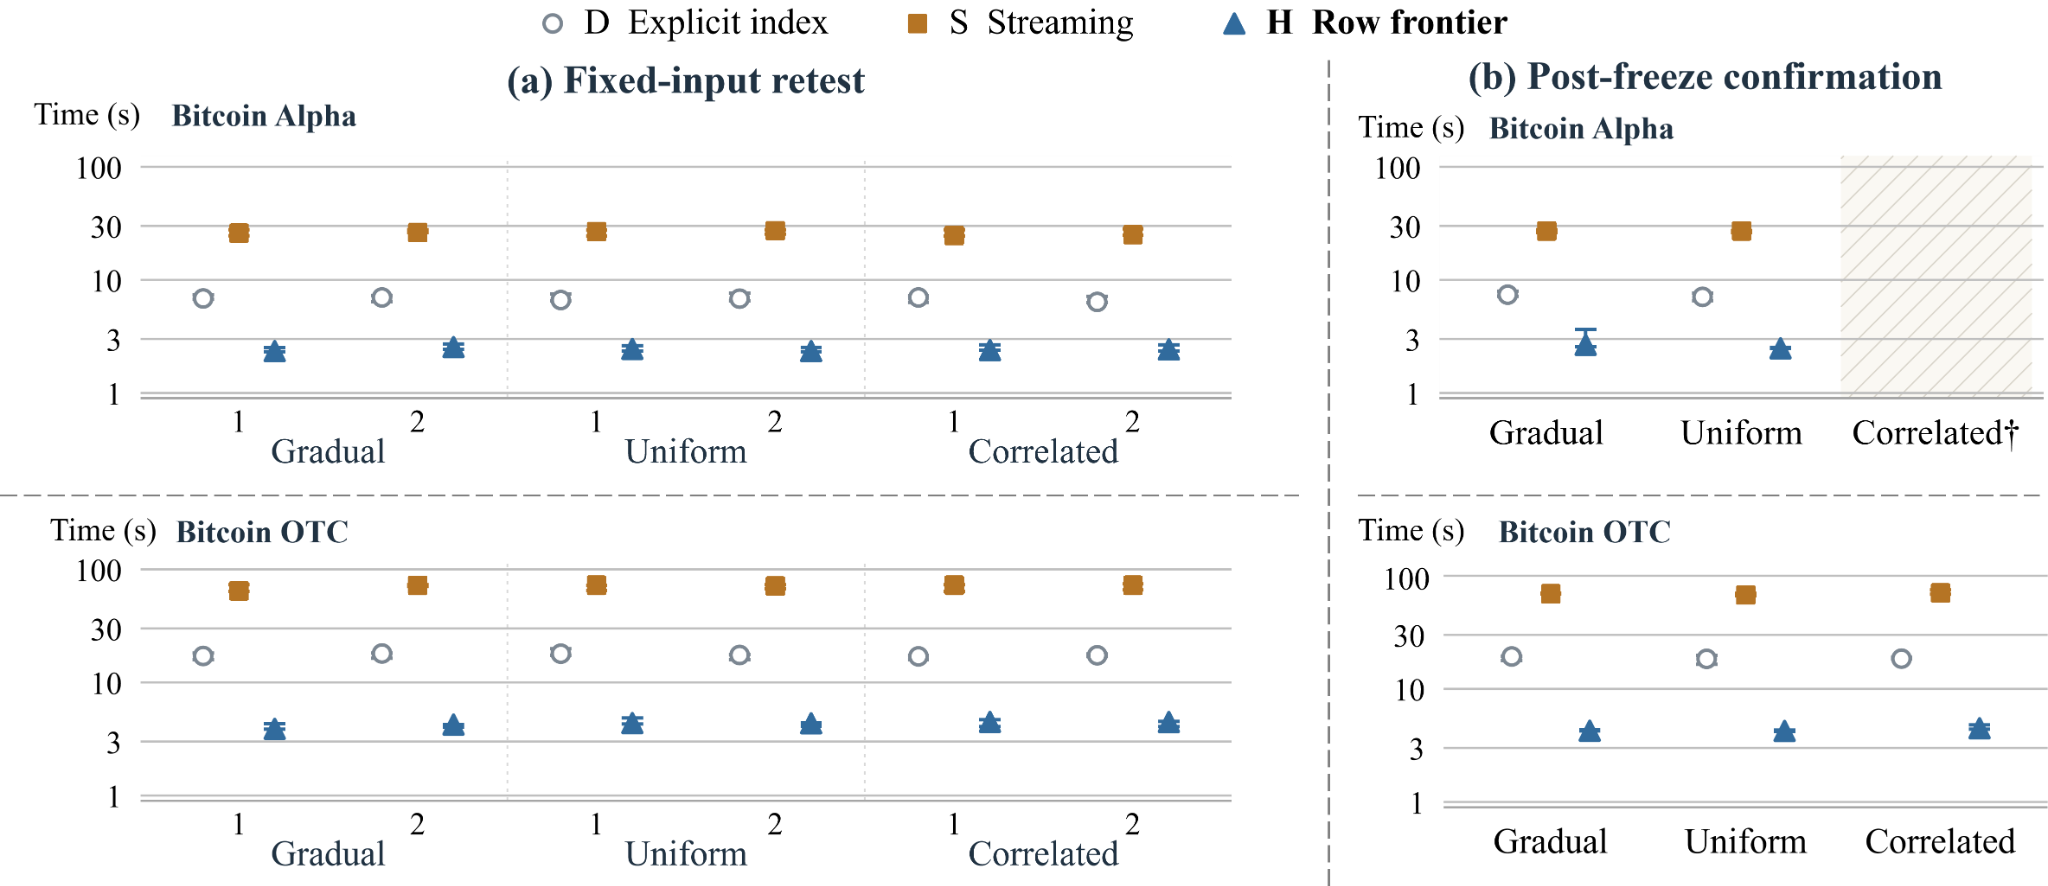
\includegraphics[width=\textwidth]{user_originals/fig2.png}
\caption{Complete setup-plus-Q4 costs of explicit indexing (D), streaming (S), and row-frontier access (H) under the original instrumented policy. (a) Twelve previously diagnosed streams, with labels 1 and 2 identifying two inputs per graph and opinion family. (b) Six streams generated after implementation freezing. Gradual, uniform, and correlated denote gradual-change, independent-uniform, and signed-neighbor opinions. Markers show medians; whiskers span three-repeat minima and maxima on logarithmic time axes. The hatched $\dagger$ cell has no complete Q4 time (Section~\ref{sec:completion}).}
\Description{Two rows show Bitcoin Alpha and OTC. The fixed-input retest appears on the left and post-freeze confirmation on the right. H has lower complete costs than D and S on the completed streams. The Alpha correlated confirmation cell is hatched and marked with a dagger because no complete Q4 timing is available.}
\label{fig:costs}
\end{figure*}

% P:HG1
\textbf{The alternative cover lowers complete cost.} Under common \texttt{light\_v1} measurement on the same five completed streams, G uses 12.56\% less aggregate service time than H: 18.833572 versus 21.537746 seconds over 15 pairs. G is faster in 14 pairs, and all five per-stream median ratios favor G (Figure~\ref{fig:hg_costs}). The following work analysis explains how cheaper coverage preparation offsets greater response demand.

\begin{figure}[t]
\centering
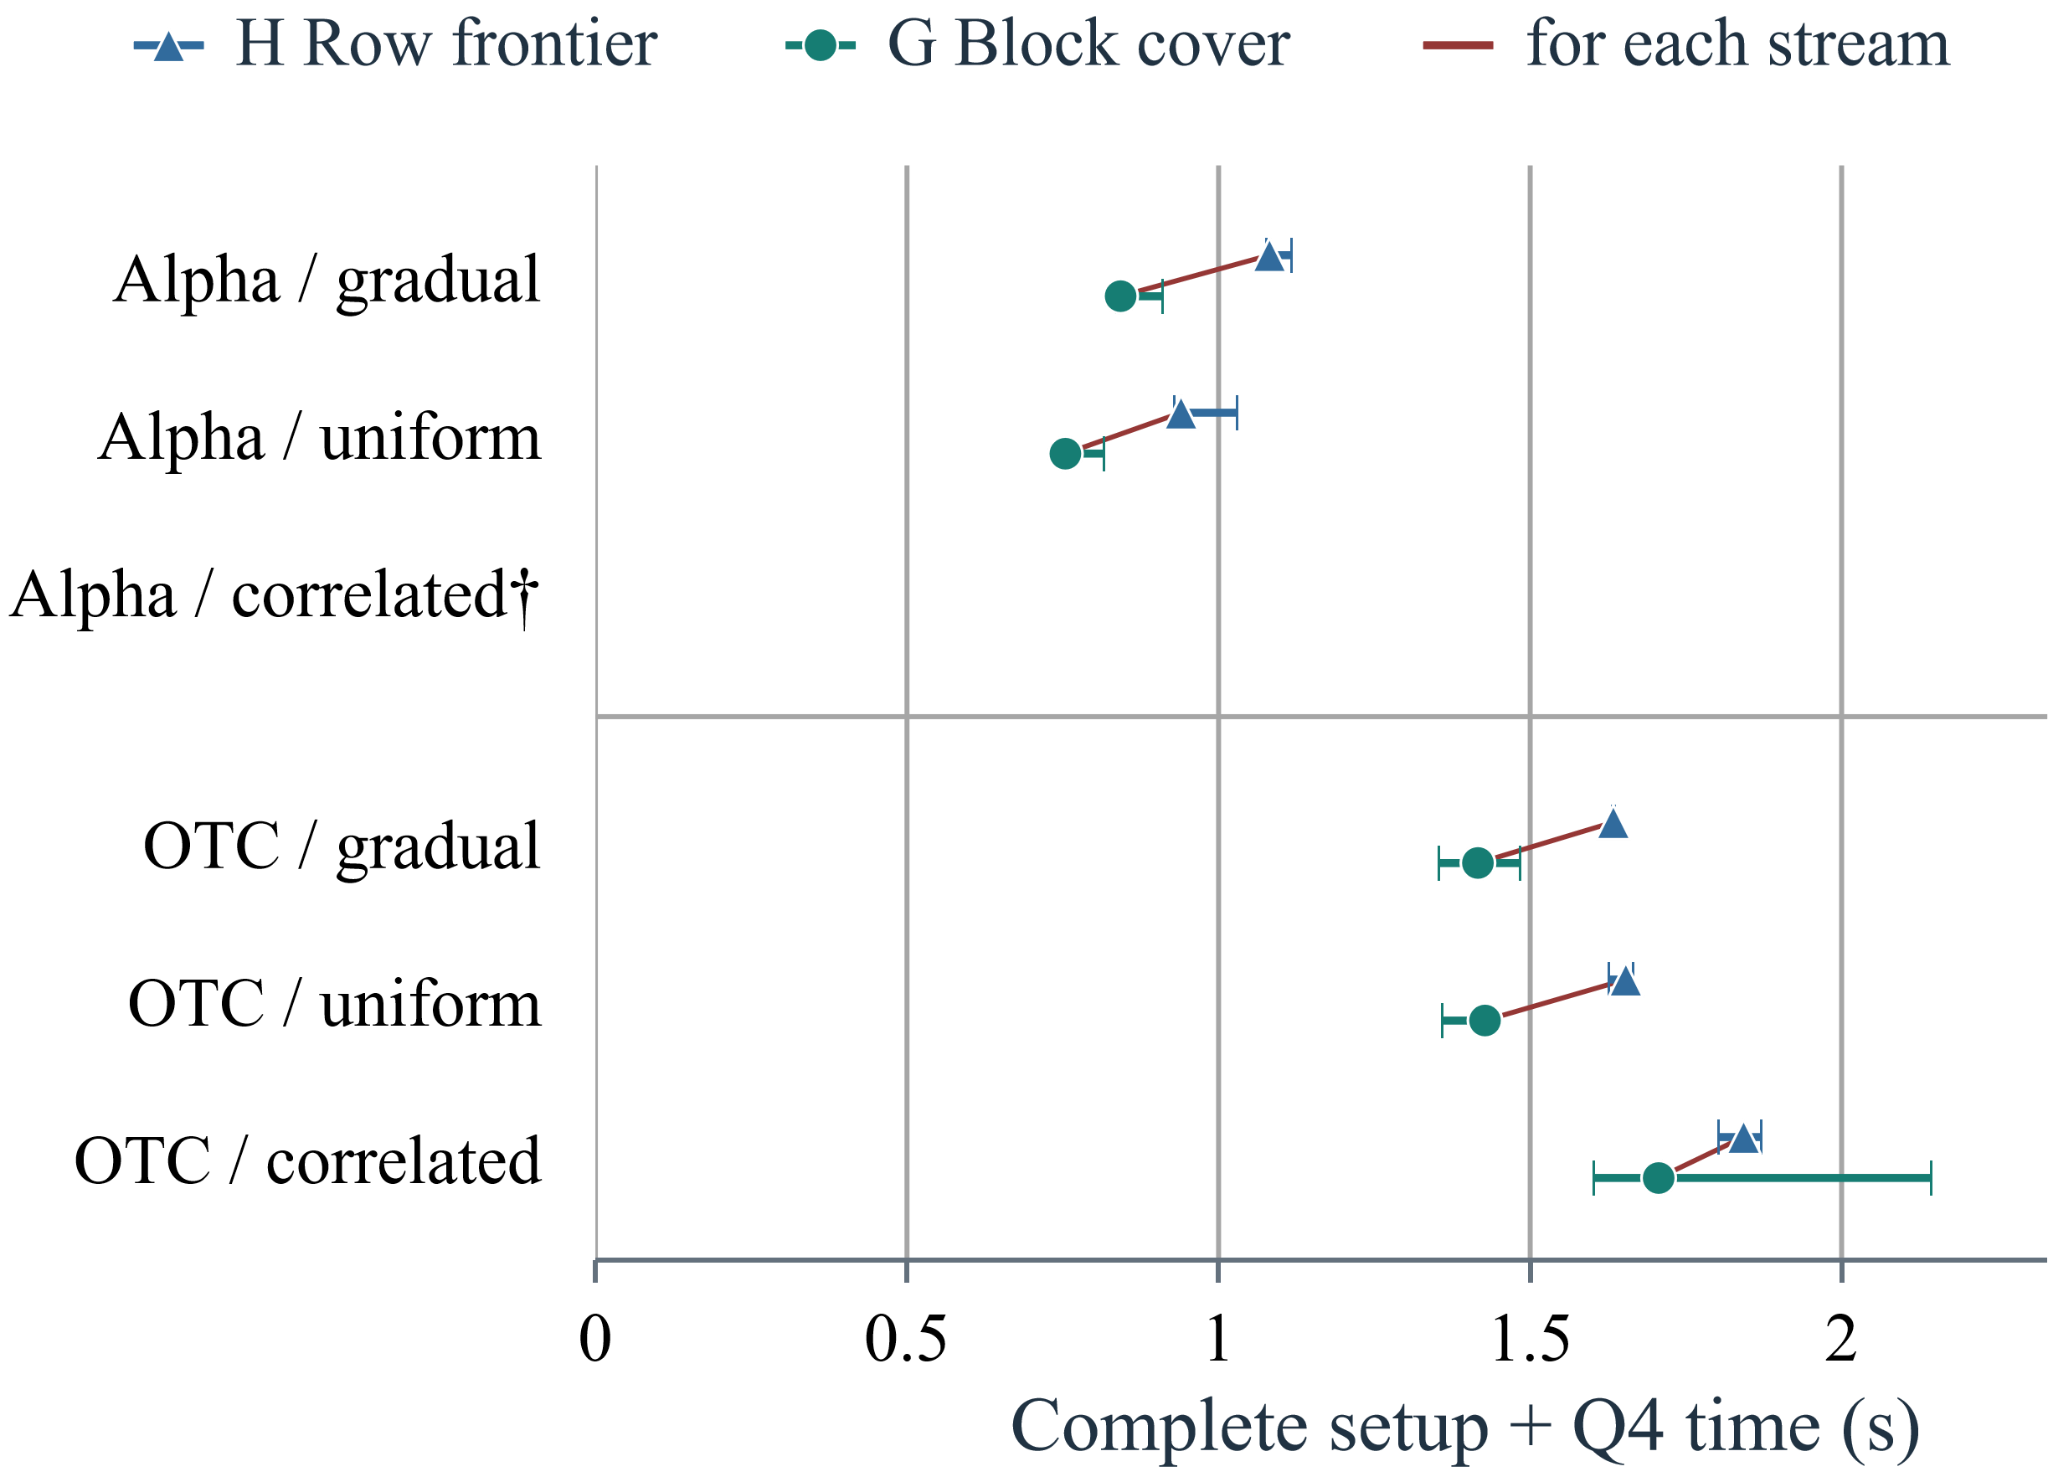
\includegraphics[width=\columnwidth]{user_originals/fig3.png}
\caption{Complete setup-plus-Q4 costs of row-frontier access (H) and block coverage (G) under common \texttt{light\_v1} measurement on the same six confirmation streams. Markers show medians; whiskers span the minimum and maximum of three timing repeats. Red segments connect H/G medians for the same stream. Opinion labels follow Figure~\ref{fig:costs}. $\dagger$ marks Alpha/correlated, for which no complete Q4 cost is available (Section~\ref{sec:completion}).}
\Description{Horizontal timing ranges compare H and G on Alpha and OTC. Blue triangles and green circles show method medians, and red segments join medians for each stream. G has a lower median in all five completed streams. The Alpha correlated stream remains as a dagger-marked row with no complete timing.}
\label{fig:hg_costs}
\end{figure}



\subsection{RQ2: Where Does Coverage Save Work?}
% P:E7
The diagnosed retest exposes an access-work difference with matching response demand: H and D have equal graph-level mean Gram and response-block counts, while D processes about 470 and 784 times as many endpoint rows on Alpha and OTC. H pays for all 60 frontier builds per completed Q4. Median peak RSS over 18 workers per graph and method is 108.45/124.76 MiB for H, versus 583.19/1,216.81 for D. Streaming uses similarly low memory to H but scans hundreds of millions to over a billion endpoint rows per Q4. Implicit representation and selective access thus address different costs. RSS includes factors, caches, and runtime objects.

% P:E8
G shifts work from coverage preparation to numerical response acquisition. Over the same 15 complete H/G pairs, it sends fewer cold rows to endpoint screening and requests more RHS columns, scores, Grams, and transfers (Table~\ref{tab:hg_work}). Cold rows count inputs to endpoint screening. Mutually exclusive phase totals for H/G are 5.936/2.258 seconds in frontier preparation, 5.582/6.115 in response acquisition, and 0.868/0.934 in transfer. The reduction in preparation cost more than offsets the additional numerical work, explaining G's lower complete-service time on these inputs.

\begin{table}[t]
\centering
\caption{Work over the 15 complete H/G pairs under \texttt{light\_v1}: 60 requests and 900 accepted records per method.}
\label{tab:hg_work}
\begin{tabular}{@{}lrr@{}}
\toprule
Recorded work & H & G\\
\midrule
Cold rows sent to screening & 6,081 & 741\\
Candidate RHS columns & 2,214 & 2,277\\
Worker scalar RHS (all roles) & 3,081 & 3,150\\
Scoring calls & 3,789 & 4,056\\
Gram materializations & 1,305 & 1,320\\
Transfer items & 3,540 & 3,777\\
\bottomrule
\end{tabular}
\end{table}

% P:E8a
The mechanism records show how G obtains its coverage. Collapsing timing repeats by graph, root, catalog, opinion, and parent identity yields 300 decision states in the completed streams. G excludes the entire insertion class in 44\% of these states and enters block access in the remaining 56\% (Table~\ref{tab:g_mechanism}). Insertions win 34\% of decisions; moreover, 66 of the 198 flip winners also enter block access. Both whole-class exclusion and block search therefore participate in the measured execution. The artifact retains the corresponding counts for all six streams.

\begin{table}[t]
\centering
\caption{G mechanisms in five complete streams: 300 distinct decision states after removing timing repetitions. The two pairs of rows are separate partitions of the same states.}
\label{tab:g_mechanism}
\begin{tabular}{@{}lrr@{}}
\toprule
Observed property & States & Share\\
\midrule
Whole insertion class excluded & 132 & 44\%\\
Block access entered & 168 & 56\%\\
\midrule
Flip selected & 198 & 66\%\\
Insertion selected & 102 & 34\%\\
\bottomrule
\end{tabular}
\end{table}

% P:S1
\textbf{Catalog storage and numerical preparation.} A startup test on Slashdot, with $82{,}140$ vertices, separates these two costs~\cite{snapslashdot,leskovec2010signed}. D's required explicit payload is estimated at 53.404 GiB, so the 4-GiB address-space preflight prevents startup. H and S avoid that allocation; their shared SuperLU root preparation reaches the 600-second limit before the first request. This test identifies numerical preparation as the remaining startup barrier; stage and memory records are in the artifact.



\subsection{RQ3: What Do Response Maintenance and Directional Bounds Save?}
% P:E9
To examine response maintenance separately from all-nonedge access, a fixed-catalog study uses supplied catalogs of 1,000/2,500 candidates and budgets of 20/40. Its six graphs are unit-signed Alpha, OTC, and Slashdot plus controlled Conflict, Bio, and Fin graphs; $\alpha=1$, edit weights are one, opinions are bounded, and $\delta=10^{-9}$. Ten isolated single-threaded repetitions on an Intel Core i7-12700H under Windows compare Jacobi-preconditioned conjugate gradient (CG) and the CHOLMOD sparse Cholesky backend~\cite{chen2008cholmod,virtanen2020scipy}. Within each backend, cold solves, within-version caching, and planned transfer share the trajectory. Each comparison pairs policies within the same backend and environment.

% P:E10
In the six-graph, 2,500-candidate, 40-commit slice, planned CG and CHOLMOD use 1,393 and 1,407 scalar response RHS columns, including winner and refresh work, versus 15,054 for cold CG. Initialization-inclusive median times on Alpha decrease from 6.29 to 0.984 seconds for CG and from 1.08 to 0.424 for CHOLMOD; on OTC they decrease from 12.4 to 1.44 and from 2.34 to 0.613. These matched-backend comparisons support maintaining requested responses in this fixed-catalog setting. The complete six-graph table remains in the artifact.

% P:E11
The directional study asks whether bounding the queried direction reduces uncertainty on the same approximate inputs. It uses 60 negative Alpha hub edges and 72 disjoint negative Bio edges at weights $1,4,16,64$. Eight settings and 20 initial-tolerance runs yield 41,744 paired events before additional refinement or reanchoring; accepted rounds include every remaining candidate, and stop rounds add no events. Table~\ref{tab:directional}'s \emph{same-state} column compares raw normwise and directional radii on identical stored states, responses, and error histories, each with its own center. Its \emph{policy-history} column compares executions at the same candidate/version whose maintained errors and reanchor histories may differ.

\begin{table}[t]
\centering
\caption{Directional stress: median ratios of recorded normwise to directional radii. Same-state pairs share approximate inputs and error histories; policy-history pairs match the candidate and version. Each row includes all recorded tolerances and events.}
\label{tab:directional}
\begin{tabular}{lrrrr}
\toprule
Graph & Weight & Events & Same state & Policy history\\
\midrule
Alpha & 1 & 1,010 & 2.94 & 2.94\\
      & 4 & 1,010 & 8.47 & 8.67\\
      & 16 & 840 & 32.12 & 47.86\\
      & 64 & 884 & 140.49 & 757.44\\
Bio   & 1 & 9,500 & 5.17 & 5.24\\
      & 4 & 9,500 & 35.82 & 38.11\\
      & 16 & 9,500 & 669.49 & 528.49\\
      & 64 & 9,500 & 32,678.41 & 7,809.73\\
\bottomrule
\end{tabular}
\end{table}

% P:E12
Directional radii are smaller in all 41,744 paired events, with the largest median reductions at high weights. In the Bio policy comparison at weight 64, budget 50, and initial CG tolerance $10^{-5}$, reanchors decrease from 2,375 to 59 and response blocks from 2,496 to 180. This connects tighter enclosures to less response maintenance on that workload. These results compare archived radius and maintenance records; the artifact documents their audit scope.

\subsection{RQ4: Which Decisions Are Independently Verified?}
\label{sec:completion}
% P:E13
The checker asks whether a reported winner has positive gain and satisfies the current comparison against every legal rival. It reconstructs the root, exact opinion, catalog, chosen set, and selected children, independently of the execution frontier. Small graphs permit exact rational evaluation. On larger graphs, any trial $x\in\R^n$ gives
\begin{equation}
 2s^\top x-x^\top Ax\le s^\top A^{-1}s
 \le2s^\top x-x^\top Ax+\|s-Ax\|_2^2.
 \label{eq:checker-energy}
\end{equation}
The difference from the lower expression is $(s-Ax)^\top A^{-1}(s-Ax)$, bounded by the squared residual since $A\succeq I$. Dyadic integer arithmetic evaluates the enclosure; CG supplies only a trial. The checker enumerates every legal pair in bounded blocks, using its own endpoint caps and child-energy bounds, and records counts and a digest of the identifier stream.

% P:E15
The checker certifies winner positivity and all-rival comparison using its own evidence, and verifies online equality witnesses through parent and opinion invariance and child conjugacy. It separately checks published intervals: containment of the exact gain on rational instances, and nonempty intersection with an independent enclosure on larger instances. The latter is an interval-consistency check; the final decision is verified with the independent bounds.

% P:E18
All 30 decisions in two preselected H requests pass independent full-catalog replay. The requests are q1 of the independent-uniform stream on each graph, using V2 repetition zero. Table~\ref{tab:verification} places these results alongside fixed-input replays and structural or record-based checks. Checker time is accounted for separately from service cost.

\begin{table}[t]
\centering
\caption{Independent replay and complementary checks. Exec. counts request executions. The G row links 90 observations to the same 30 states replayed for H; verification populations can overlap.}
\label{tab:verification}
\begin{tabularx}{\columnwidth}{lrrY}
\toprule
Check & Exec. & Records & Scope\\
\midrule
Diagnosed fixed inputs & 10 & 150 & Full-domain replay\\
Fixed timed OTC & 1 & 15 & Full-domain replay\\
Fixed timed chains & 432 & 6,480 & Bindings and structural equality\\
V2 preselected H & 2 & 30 & Full-domain replay\\
V4 request records & 144 & 2,088 & Recorded agreement\\
G archive-derived & 6 & 90 & Interval containment\\
\bottomrule
\end{tabularx}
\end{table}

% P:E18a
\textbf{Linking the replay to G.} The same 30 replayed states support a derived check of G's published gains. Original inputs and recorded chains bind the graph, opinion, parent state, legal domain, and winner. Across three G repeats, all 90 observations satisfy $I_{\rm independent}\subseteq I_G$: the published interval contains the archived independent enclosure. This checks G's outputs at matched states, rather than independently replaying its block-pruning decisions.

% P:E19
\textbf{A structural explanation for the Alpha overlap.} An offline witness combines two vertex swaps that preserve the current parent and opinion and map the two specified children, proving equal gains. This establishes the candidate pair's exact equality. The online resolver supports single-swap witnesses, so the complete decision remains unresolved after three accepted edits. The artifact records the permutation and its bindings.

\section{Related Work and Positioning}
\label{sec:related}

% P:L1
\textbf{Ranked access and unseen candidates.} The Threshold Algorithm combines sorted and random access with a threshold for unseen objects~\cite{fagin2001aggregation}. Rank-Join and subsequent top-$k$ join processing bound unseen or partially evaluated combinations~\cite{ilyas2003rankjoin,wu2010topkjoin}. For full acyclic joins with inequality predicates, factorized representations support ranked enumeration by sums of input-tuple weights without materializing the full result~\cite{tziavelis2021beyondequijoins}. Bounds also guide the acquisition of costly scores: Bruno et al. choose candidate probes using score bounds and source-access costs~\cite{bruno2002webtopk}, while Guo et al. summarize scoring functions over query-parameter intervals to avoid unnecessary evaluations~\cite{guo2008querydependent}. H and G bring selective access to a ranking whose scores change through a graph linear system. Their coverage accounts jointly for the current legal catalog and uncertainty in computed gains.

% P:L2
\textbf{Incremental analytical state.} Retained state trades storage for cheaper subsequent work. Yi et al. maintain extra ranked tuples to reduce top-$k$ view refills after updates~\cite{yi2003topkviews}. DBToaster maintains higher-order delta views~\cite{Koch_2014}; LINVIEW propagates factored changes through linear-algebra programs~\cite{Nikolic2014Linview}; F-IVM maintains factorized relational views~\cite{kara2024fivm}. REX carries this principle into recursive analytics by propagating deltas and updating operator state between iterations~\cite{mihaylov2012rex}.

% P:L2a
In graph processing, Ingress chooses among memoization policies~\cite{gong2021ingress}, and Layph constrains change propagation through a layered graph~\cite{yu2023layph}. Selective reuse also supports concurrent queries: KGraph memoizes pivot-query results within graph partitions~\cite{gao2025kgraph}, while Aquila shares common subgraph work in continuous pattern matching~\cite{zou2025aquila}. J-CERT+ retains requested endpoint Grams with error bounds and version bindings, then couples their reuse to coverage of the current intervention catalog.

% P:L3
\textbf{Inverse information on graphs.} Precomputed graph coordinates support fast approximate hitting-time, commute-time, and personalized PageRank queries~\cite{zhao2013randomwalk}. For effective resistance, Liao et al. maintain random-walk and loop-erased-walk samples after graph updates~\cite{liao2025resistance}; Yang et al. develop Lanczos iteration and local-push algorithms for pair queries~\cite{yang2026resistance}. Forest sampling and Schur complements estimate grounded-Laplacian inverse quantities for approximate current-flow group-closeness maximization~\cite{xia2025groupcloseness}. Related forest methods estimate evolving forest-matrix entries, opinion quantities, and signed forest diagonals~\cite{sun2024evolving,sun2025opinion,sun2026signed}. At the numerical layer, dynamic Cholesky maintains sparse factors~\cite{davis2009dynamic}, selected inversion computes entries associated with a factor's pattern~\cite{lin2011selinv}, and matrix quadrature bounds inverse forms~\cite{li2016quadrature}. J-CERT+ uses local projections of a shifted signed operator to certify edit gains and transport their numerical evidence.

% P:L4
\textbf{Graph interventions and opinion dynamics.} Prior work optimizes links for polarization and disagreement~\cite{musco2018polarization,zhu2021polarization}, and local edge dynamics use rank-one insertion identities~\cite{bhalla2023local}. SPGREEDY computes each greedy insertion argmax in exact arithmetic; FASTGREEDY further approximates candidate effects~\cite{zhu2021polarization}. Liu et al. study edge addition for resistance-based fairness in information access, using greedy gain evaluation and low-rank inverse updates~\cite{liu2026accessfairness}. Other opinion interventions select seed users for competing campaigns at a finite horizon~\cite{saha2025voting}, or modify initial opinions in signed Friedkin--Johnsen models~\cite{zhou2024signedfj}. J-CERT+ addresses a mixed insertion-and-flip catalog and certifies each current choice with finite-precision positivity, coverage, and canonical-tie requirements.

% P:L5
\textbf{Reliable numerical outputs.} Residual-based output correction supplies the identity behind our directional center~\cite{BalabanovNouy2019}; normwise Woodbury analysis studies related reliability questions~\cite{MaEtAl2026}. J-CERT+ combines these numerical tools with pivot bounds derived from legal edits, input and arithmetic allowances, and propagated Gram errors. Exact conjugacy supplies equality evidence when independent intervals overlap.

\section{Conclusion}
\label{sec:conclusion}
% P:Z1
J-CERT+ makes complete candidate coverage compatible with selective numerical work. Certified transfer carries useful endpoint summaries across graph edits, while row and block access paths establish the current bounds needed to choose among legal alternatives. The Alpha/OTC experiments show that implicit access reduces complete service cost and that alternative coverage structures trade preparation work against response demand. Independent replay checks selected decisions against the full catalog. Separating reusable response state from current coverage gives the service a common certification contract across distinct access organizations.

\appendix
\section{Arithmetic and Precision Details}
\label{app:arithmetic}

% P:A1
For the allowances in Section~\ref{sec:numerics}, assume finite represented inputs with no overflow or unaccounted underflow. Let $u=2^{-53}$ be the binary64 unit roundoff, $\gamma_k=ku/(1-ku)$ for $ku<1$, and $\mathcal N$ be an outward upper Euclidean or Frobenius norm~\cite{Higham2002}. Write $\mathcal P_k(X,Y)=\gamma_k\mathcal N(X)\mathcal N(Y)$ and $\mathcal S(X,Y)=\gamma_1\mathcal N(|X|+|Y|)$. For input radii $R_X,R_Y$ and a product with inner dimension $k$, product and sum errors propagate by
\begin{equation}
 \begin{aligned}
 R_{XY}&=\mathcal N(\widetilde X)R_Y+\mathcal N(\widetilde Y)R_X\\
       &\qquad+R_XR_Y+\mathcal P_k(\widetilde X,\widetilde Y),\\
 R_{X\pm Y}&=R_X+R_Y+\mathcal S(\widetilde X,\widetilde Y).
 \end{aligned}
 \label{eq:rounding}
\end{equation}
Starting with zero radii on represented center operands isolates arithmetic error in center evaluation, symmetrization, and trial residuals. For example, for an $r\times r$ pivot with $P_B=\fl(\widetilde B\widetilde T)$, use $\eta_T=\mathcal N(\fl(I-P_B))+\mathcal P_r(\widetilde B,\widetilde T)+\mathcal S(I,P_B)$. The operators $\down$ and $\up$ round downward and upward. Final endpoints are $\down(\widehat g-R)$ and $\up(\widehat g+R)$, with their outward-rounding excess included in the reported complete radius~\cite{Rump2010}.

% P:A2
To turn a computed residual into a state-error bound, let $\widehat r=\fl(\widetilde A\widetilde x-\widetilde b)$. For row length $d_i$ and entrywise input-error bounds $\Delta A,\Delta b$, each component of the true residual is bounded in magnitude by
\begin{equation}
 \begin{aligned}
 q_i=\up\!\big[&|\widehat r_i|+
 \gamma_{d_i+5}(|\widetilde A||\widetilde x|+|\widetilde b|)_i\\
 &+(\Delta A|\widetilde x|+\Delta b)_i\big].
 \end{aligned}
 \label{eq:residual}
\end{equation}
Here $q$ is the residual-bound vector, local to this appendix. The contraction bounds of Section~\ref{sec:contract} make $\mathcal N(q)$ and $\max_iq_i$ state-error bounds in the Euclidean and maximum norms. Response columns obey the same contraction, with column bounds combined in Frobenius norm. Assume assembled $\widetilde U$ preserves the exact basis's two-endpoint support $Q$. If $E_U\ge\|U-\widetilde U\|_2$ and the residual against $\widetilde U$ yields $\bar r\ge\|A^{-1}\widetilde U-\widetilde Y\|_2$, endpoint contraction gives
\begin{equation}
 \begin{aligned}
 E_G={}&\|U\|_2(\bar r+E_U)+E_U\|\widetilde Y_Q\|_2\\
 &+\mathcal P_2(\widetilde U_Q^\top,\widetilde Y_Q).
 \end{aligned}
 \label{eq:gram-error}
\end{equation}
Expanding the corresponding products gives projection and cross-response errors by the same reasoning. On two endpoint rows, a state two-norm bound can be tightened to the minimum of its global two-norm bound and $\sqrt2$ times its maximum-norm bound; for a rank-$r_a$ response block use $\sqrt{2r_a}$. The integer normalized basis sets $E_U=0$. Applying these allowances to state perturbation and local inversion also certifies the endpoint screens used for coverage.

% P:A7
The main service binds fixed-point integers to physical gain units. Opinion numerators have denominator $2^{16}$, and the stored integer operator is $16A_T$. The fine proof grid uses coefficient denominator $2^{48}$. Raw score integers $L_{\rm raw},U_{\rm raw}$ use denominator $2^{96}$; multiplying each by $16/2^{96}$ gives the physical gain endpoints. Published decision numerators already include the factor 16. Equality witnesses bind these conventions to the current operator and opinion, keeping the relation and gain intervals in the same units.

\subsection{Proof of Theorem~\ref{thm:finite}}
\label{app:finite}

% P:A3
We first bound error through $b$ transfers using the normwise enclosure; any valid tighter enclosure may be retained. Maximum-norm contraction, endpoint support, and~\eqref{eq:gram-error} give
\[
 E_G(0)\le(3k+1+2\eps)\eps\le(a_0-1)\eps,
 \quad E_C,E_h\le a_0\eps,
\]
and $\|\widetilde C\|_2\le c_0$, $\|\widetilde h\|_2\le\bar h$. Each input, true-residual, and complete local allowance uses the theorem's common $\eps$ in its stated norm.

% P:A4
First control the inverse trial used in each local update. Let $R_T=I-\widetilde B\widetilde T$. Equation~\eqref{eq:inverse-error} and the triangle inequality imply
\[
 (1-\beta E_B)\|\widetilde T\|_2
 \le\beta(1+\|R_T\|_2).
\]
Whenever $E_B\le H_b\eps$,~\eqref{eq:finite-eps} makes the left coefficient at least $3/4$; with $\|R_T\|_2\le\eps\le1/4$, this gives $\|\widetilde T\|_2<2\beta$. The policy constructs the winner pivot from its current certified transition-response block, so its stronger fresh bound is $E_{B,a}\le a_0\eps$. Thus $E_{T,a}\le t_0\eps$. Substituting $E_C\le a_0\eps$, $\|\widetilde C\|_2\le c_0$, and $\eps\le1$ into~\eqref{eq:normwise} shows that one transfer increases a Gram radius by at most $\ell_0\eps$.

% P:A5
The single-transfer bound now closes the induction: $E_G(j)\le(a_0-1+j\ell_0)\eps$ after $j\le b$ commits. Adding pivot assembly gives $E_B\le H_b\eps$, so the inverse-trial premise continues to hold at every reached version. Equations~\eqref{eq:inverse-error} and~\eqref{eq:normwise} then give every competitive score a complete radius at most $F_0\eps\le\delta/8$, hence interval width at most $\delta/4$.

% P:A6
For the decision, retain valid unseen and endpoint exclusions; an undischargeable upper bound supplies no narrow score interval. By finite complete access, materialize and score every remaining candidate whose bound has not been discharged by a current decision cut; conservatively scoring the entire remaining catalog terminates because it is finite. Now every undiscarded candidate has the width bound proved above. If all remaining upper gains are at most $\delta$, the contract permits a tolerance stop. Otherwise a scored interval has $u_e>\delta$, hence $\ell_e>3\delta/4$. Choosing the largest competitive lower endpoint gives $\ell_a>0$ and $u_e\le\ell_e+\delta/4\le\ell_a+\delta/4$ for every other competitive edit. Excluded candidates remain covered by their certified cuts. Thus acceptance or stopping requires no inherited-view numerical reanchor. Charge one first response block for each of the $N$ materialized candidates and at most one current transition block per commit, reusing qualifying resident blocks. This proves the response-block bound $N+b$. The number $N$ may reach catalog size; state certification, coverage, local transfer, and checker work remain outside the count.


\begin{acks}
% P:AK1
\noindent\textbf{Declaration on the use of generative AI tools}\par
Generative AI tools were used only for language polishing and grammar checking during the preparation of this manuscript. The authors reviewed and verified all AI-assisted edits and take full responsibility for the content of the manuscript.\label{last-body-page}
\end{acks}

% The class balances the last reference page through its standard end hook.
\bibliographystyle{ACM-Reference-Format}
\bibliography{references}
\end{document}
